% Provenance (never printed): see sources/outline_sources.md (Year 1: stress and
% principal stresses in 2D; strain; pure and simple shear; elastic, brittle and ductile
% behaviour; the strength envelope of the lithosphere). Strength envelopes from
% figdata/bachelor-1/strength_envelope.py (Byerlee 1975; flow laws of Gleason and Tullis
% 1995 and Hirth and Kohlstedt 2003 as compiled by Lopez-Sanchez; geotherms of ch. 10);
% exercise and problem values in the Book 3 scratch calculator calc/ch16.py. Traction,
% shear stress, the stress and strain tensors, Hooke's law, Young's modulus and viscosity
% belong to the physics series and are recalled, never defined (sync 1 ruling).
\chapter{الإجهاد والانفعال والريولوجيا}\label{ch:b1:stress-strain-rheology}

في ستينيات القرن العشرين، تسرّب سائل النفايات المضخوخ في بئر تصريف في مخزن روكي ماونتن أرسنال، قرب دنفر، عبر قاعدة بلورية متشققة بين \qty{3.7}{km} و\qty{7.0}{km} تحت السطح، وتلتها زلازل. وبقيت داخل الجزء من الصخر الذي ارتفع فيه ضغط السائل بأكثر من نحو \qty{3.2}{MPa}.
% ledger: hb81:denver
بعد نصف قرن حدث الشيء نفسه على نطاق أوسع في أوكلاهوما، حيث يُعاد ضخ الماء المالح المصاحب للنفط والغاز تحت الأرض. وفي الولاية وحولها، كان عدد الزلازل ذات القوة 3 فأكثر بين واحد وخمسة في السنة من 2005 إلى 2008، ثم 20 في 2009، و\num{585} في 2014، و\num{888} في 2015، أي أكثر من اثنين في اليوم؛ وهزّت هزّتان بقوة 5.7 و\num{5.8} براغ عام 2011، وباوني عام 2016. ويمكن لأربعة آبار تصريف عالية الحجم وحدها أن تفسّر خُمس زلازل وسط الولايات المتحدة، وأن تُطلق بعضها على أكثر من \qty{30}{km} بعيدًا.
% ledger: usgs:oklahoma-rate, usgs:prague-pawnee, keranen:oklahoma
لم يدفع الماء شيئًا جانبًا؛ بل رفع فقط ضغط السائل في مسامّ الصخر. فلماذا ينبغي لذلك أن يجعل صدعًا ينزلق؟ الجواب يحتاج إلى ثلاث أفكار، هي موضوع هذا الفصل: الإجهاد على مستوٍ داخل الصخر، والشرط الذي ينهار عنده المستوى، وأن \omterm{def:b1:stress-strain-rheology:lithostatic}{ضغط سائل المسام} يعاكس القوة التي تضغط الجانبين معًا. ومع هذه الأفكار، ومع قانون زحف للصخر الحار، يمكن أن نرسم مقاومة \omterm{def:b1:layered-earth:lithosphere}{الغلاف الصخري} كله بدلالة العمق.

\begin{recall}
تُطبَّق القوة الموزعة على سطح بقوتها لكل وحدة مساحة، بالباسكال؛ ويزداد الضغط في مائع ساكن مع العمق وفق $\rho g z$ (كتب الفيزياء). ويطيع النابض، والجسم الصلب في التشوّهات الصغيرة، قانون هوك: الانفعال متناسب مع الإجهاد، وثابت التناسب هو معامل يونغ؛ والمائع اللزج يقاوم بتناسب مع معدّل قصّه، وثابته هو اللزوجة. ويصف كتاب الفيزياء للسنة الجامعية الثالثة الإجهاد والانفعال في ثلاثة أبعاد بالموتّرات؛ وهذا الفصل يحتاج بعدين فقط. والمصفوفة المتماثلة $2\times2$ لها قيمتان ذاتيتان حقيقيتان ومتجهتان ذاتيتان متعامدتان (الرياضيات). وتعطي المنحنيات الحرارية في \cref{ch:b1:heat-budget} درجة الحرارة عند العمق؛ وقد لُقيت الصدوع في الكتاب 1، الصف 7.
\end{recall}

\section{الإجهاد في بعدين}\label{sec:b1:stress-strain-rheology:stress}

لنقطع صخرًا بالفكر على سطح مستوٍ صغير. فالصخر في جانب يضغط على الصخر في الجانب الآخر بقوة، والقوة لكل وحدة مساحة هي «الجهد» على ذلك السطح، بلغة كتب الفيزياء. واتجاهها ليس، في العموم، اتجاه العمودي على السطح.

\begin{definition}[الإجهاد العمودي]\label{def:b1:stress-strain-rheology:stress}
على مستوٍ يمرّ بنقطة من الصخر، تملك القوة لكل وحدة مساحة التي يؤثّر بها الصخر في جانب على الجانب الآخر مركّبةً على العمودي على المستوى، هي \emph{الإجهاد العمودي}\index{الإجهاد العمودي} $\sigma_n$، ومركّبةً على المستوى، هي إجهاد القص $\tau$. وفي علوم الأرض يُعدّ الإجهاد العمودي موجبًا حين يضغط.
\end{definition}

وإشارة الاتفاق معاكسة لإشارة المهندس. وقد اختيرت لأن كل إجهاد تقريبًا في الأرض الصلبة ضغط: فثقل الصخر فوق يضغط على كل ما هو أسفله.

نعمل في مستوٍ شاقولي، بمحور $x$ أفقي ومحور $y$. وعلى مستوٍ عمودي على $x$ يكون \omterm{def:b1:stress-strain-rheology:stress}{الإجهاد العمودي} $\sigma_{xx}$ وإجهاد القص $\sigma_{xy}$؛ وعلى مستوٍ عمودي على $y$ يكونان $\sigma_{yy}$ و$\sigma_{yx}$. وإجهادا القص متساويان: ففي مربع صغير، تصنع قوى القص على الجانبين الشاقوليين مزدوجة عزمها $\sigma_{xy}a\cdot a$ لجانب طوله $a$، وتلك على الجانبين الأفقيين مزدوجة $\sigma_{yx}a\cdot a$ تدور في الاتجاه المعاكس، ويدور المربع لو اختلفتا. فثلاثة أعداد تصف الإجهاد عند نقطة، وهي تكفي لإعطائه على كل مستوٍ.

\begin{proposition}[الإجهاد على مستوٍ مائل]\label{prop:b1:stress-strain-rheology:transformation}
لنأخذ مستوًى ذا متجهة العمودي الوحدة $\vec n = (\cos\theta, \sin\theta)$، بزاوية $\theta$ من المحور $x$، ولتكن $\vec m = (-\sin\theta, \cos\theta)$ متجهة الوحدة على امتداد المستوى. فالإجهادان العمودي والقصّي عليه هما
\begin{align*}
  \sigma_n &= \sigma_{xx}\cos^2\theta + 2\sigma_{xy}\sin\theta\cos\theta + \sigma_{yy}\sin^2\theta
           = \frac{\sigma_{xx}+\sigma_{yy}}{2} + \frac{\sigma_{xx}-\sigma_{yy}}{2}\cos2\theta + \sigma_{xy}\sin2\theta, \\
  \tau     &= (\sigma_{yy}-\sigma_{xx})\sin\theta\cos\theta + \sigma_{xy}(\cos^2\theta - \sin^2\theta)
           = -\frac{\sigma_{xx}-\sigma_{yy}}{2}\sin2\theta + \sigma_{xy}\cos2\theta ,
\end{align*}
مع احتساب $\tau$ موجبًا على امتداد $\vec m$.
\end{proposition}

\begin{proof}
لنقتطع منشورًا صغيرًا، كما في الشكل أدناه: وجه مائل مساحته $A$ ومتجهة عموديه الخارجية $\vec n$، ووجه شاقولي مساحته $A\cos\theta$، ووجه أفقي مساحته $A\sin\theta$، لكل وحدة طول في الاتجاه الثالث. ووزنه وقصوره القصوري يتناسبان مع حجمه، والحجم يتقلّص أسرع من أوجهه؛ فلمنشور صغير بما يكفي، يجب أن تتوازن القوى على أوجهه وحدها. ولأن الضغط موجب، يدفع الصخر الخارجي على الوجه الشاقولي بالقوة $A\cos\theta\,(\sigma_{xx}, \sigma_{xy})$، وعلى الوجه الأفقي بالقوة $A\sin\theta\,(\sigma_{xy}, \sigma_{yy})$؛ وعلى الوجه المائل يدفع بالقوة $-A(\sigma_n\vec n + \tau\vec m)$. ومجموعها صفر:
\[
  \sigma_n\vec n + \tau\vec m = \cos\theta\,(\sigma_{xx}, \sigma_{xy}) + \sin\theta\,(\sigma_{xy}, \sigma_{yy}) .
\]
الجداء القياسي مع $\vec n$ يعطي $\sigma_n$، ومع $\vec m$ يعطي $\tau$، لأن $\vec n\cdot\vec m = 0$. وتأتي الصيغ الثانية من $\cos^2\theta = (1+\cos2\theta)/2$، و$\sin^2\theta = (1-\cos2\theta)/2$، و$2\sin\theta\cos\theta = \sin2\theta$.
\end{proof}

\begin{omfigure}
\begin{tikzpicture}[>={Stealth[length=5pt]}, font=\small]
% theta = 35 deg, hypotenuse L = 4.5: a = L cos(theta), b = L sin(theta)
\pgfmathsetmacro{\th}{35}
\pgfmathsetmacro{\L}{4.5}
\pgfmathsetmacro{\a}{\L*cos(\th)}
\pgfmathsetmacro{\b}{\L*sin(\th)}
\coordinate (O) at (0,0);
\coordinate (A) at (0,\a);
\coordinate (B) at (\b,0);
\coordinate (M) at ($(A)!0.5!(B)$);
\fill[omLithGranite!45] (O) -- (A) -- (B) -- cycle;
\draw[line width=0.8pt] (O) -- (A) -- (B) -- cycle;
% axes
\draw[->, black!70] (-2.6,-1.9) -- (-1.6,-1.9) node[right] {$x$};
\draw[->, black!70] (-2.6,-1.9) -- (-2.6,-0.9) node[above] {$y$};
% face on x = 0 (outward normal -x), area A cos(theta)
\draw[->, line width=1.1pt, omDef] (-1.35,0.5*\a) -- (-0.05,0.5*\a);
\node[omDef, anchor=south] at (-0.95,0.5*\a+0.05) {$\sigma_{xx} A\cos\theta$};
\draw[->, line width=1.1pt, omProp] (-0.25,0.5*\a-1.25) -- (-0.25,0.5*\a-0.25);
\node[omProp, anchor=east] at (-0.3,0.5*\a-0.85) {$\sigma_{xy} A\cos\theta$};
% face on y = 0 (outward normal -y), area A sin(theta)
\draw[->, line width=1.1pt, omDef] (0.68*\b,-1.35) -- (0.68*\b,-0.05);
\node[omDef, anchor=west] at (0.68*\b+0.05,-1.05) {$\sigma_{yy} A\sin\theta$};
\draw[->, line width=1.1pt, omProp] (0.1,-0.25) -- (1.1,-0.25);
\node[omProp, anchor=north east] at (0.9,-0.32) {$\sigma_{xy} A\sin\theta$};
% inclined face, area A, normal n = (cos theta, sin theta)
\draw[->, line width=1.1pt, omThm] ($(M)+(\th:1.5)$) -- ($(M)+(\th:0.05)$);
\node[omThm, anchor=south west, inner sep=1pt] at ($(M)+(\th:1.5)$) {$\sigma_n A$};
\draw[->, line width=1.1pt, omThm!70!black] ($(M)+(\th:0.25)+(\th-90:0.75)$) -- ($(M)+(\th:0.25)+(\th-90:1.75)$);
\node[omThm!70!black, anchor=west] at ($(M)+(\th:0.3)+(\th-90:1.3)$) {$\tau A$};
\draw[->, black!70, dashed] ($(M)+(\th+90:1.25)$) -- ++(\th:1.0) node[pos=1, anchor=south west, inner sep=1pt, text=black] {$\boldsymbol n$};
% angle theta at A, between the face and the y axis
\pic[draw, angle radius=0.75cm, pic text={$\theta$}, angle eccentricity=1.35] {angle = O--A--B};
\end{tikzpicture}
\par\smallskip{\small توازن القوى على منشور صغير مثلثي من الصخر. الوجه المائل مساحته $A$ وعموديه الوحدة $\vec n$؛ والوجهان الشاقولي والأفقي مساحتاهما $A\cos\theta$ و$A\sin\theta$. الأزرق: القوى العمودية على الوجهين الصغيرين؛ البرتقالي: قوى القص عليهما؛ الأحمر: القوى العمودية وقوى القص على الوجه المائل. يُحسب الضغط موجبًا، فتشير كل قوة عمودية نحو داخل المنشور.}
\label{fig:b1:stress-strain-rheology:prism}
\end{omfigure}

\begin{theorem}[الإجهادات الرئيسية]\label{thm:b1:stress-strain-rheology:principal}
عند كل نقطة من الصخر يوجد مستويان متعامدان يكون فيهما إجهاد القص معدومًا. والإجهادان العموديان عليهما هما الأكبر والأصغر من بين كل الإجهادات العمودية على المستويات المارّة بالنقطة،
\[
  \sigma_{1,3} = \frac{\sigma_{xx}+\sigma_{yy}}{2} \pm
  \sqrt{\Bigl(\frac{\sigma_{xx}-\sigma_{yy}}{2}\Bigr)^2 + \sigma_{xy}^2},
  \qquad \tan2\theta_p = \frac{2\sigma_{xy}}{\sigma_{xx}-\sigma_{yy}},
\]
حيث $\theta_p$ الزاوية من المحور $x$ إلى عمودي المستوى الذي يحمل $\sigma_1$.
\end{theorem}

\begin{proof}
نكتب $c = (\sigma_{xx}+\sigma_{yy})/2$، ونختار $R \ge 0$ و$\theta_p$ بحيث $(\sigma_{xx}-\sigma_{yy})/2 = R\cos2\theta_p$ و$\sigma_{xy} = R\sin2\theta_p$؛ فيكون $R = \sqrt{((\sigma_{xx}-\sigma_{yy})/2)^2 + \sigma_{xy}^2}$ و$\tan2\theta_p$ كما هو مذكور. وتصبح الصيغ الثانية في \cref{prop:b1:stress-strain-rheology:transformation} هي
\[
  \sigma_n = c + R\cos(2\theta - 2\theta_p), \qquad \tau = -R\sin(2\theta - 2\theta_p).
\]
\omterm{def:b1:stress-strain-rheology:stress}{والإجهاد العمودي} أكبر ما يكون، أي $c + R$، عند $\theta = \theta_p$، وأصغر ما يكون، $c - R$، عند $\theta = \theta_p + \ang{90}$؛ وعندهما يكون $\tau = 0$. ولاحظ أيضًا أن $\mathrm d\sigma_n/\mathrm d\theta = 2\tau$: \omterm{def:b1:stress-strain-rheology:stress}{فالإجهاد العمودي} ساكن بالضبط حيث ينعدم إجهاد القص.
\end{proof}

\begin{definition}[الإجهادات الرئيسية؛ الإجهاد التفاضلي]\label{def:b1:stress-strain-rheology:principal}
\emph{الإجهادات الرئيسية}\index{الإجهادات الرئيسية} عند نقطة هي الإجهادات العمودية $\sigma_1 \ge \sigma_3$ على المستويين الخاليين من إجهاد القص، واتجاهاتها هي الاتجاهات الرئيسية. وفي ثلاثة أبعاد توجد ثلاثة، $\sigma_1 \ge \sigma_2 \ge \sigma_3$، على ثلاثة مستويات متعامدة. و\emph{الإجهاد التفاضلي}\index{الإجهاد التفاضلي} هو $\sigma_1 - \sigma_3$، والإجهاد المتوسط في المستوى هو $(\sigma_1+\sigma_3)/2$.
\end{definition}

أسهل قراءة لحالة الإجهاد تكون في اتجاهاتها الرئيسية. فإذا قِسنا الزاوية $\theta$ من اتجاه $\sigma_1$ بدلًا من المحور $x$، تفقد الصيغ حدّيها الأخيرين.

\begin{proposition}[دائرة موهر]\label{prop:b1:stress-strain-rheology:mohr}
على مستوٍ يصنع عموديه الزاوية $\theta$ مع اتجاه $\sigma_1$،
\[
  \sigma_n = \frac{\sigma_1+\sigma_3}{2} + \frac{\sigma_1-\sigma_3}{2}\cos2\theta,
  \qquad
  |\tau| = \frac{\sigma_1-\sigma_3}{2}\,|\sin2\theta| .
\]
كلّما دار $\theta$ انتقلت النقطة $(\sigma_n, |\tau|)$ على النصف العلوي من الدائرة التي مركزها $((\sigma_1+\sigma_3)/2,\, 0)$ ونصف قطرها $(\sigma_1-\sigma_3)/2$، عند الزاوية $2\theta$ من طرفها $\sigma_1$. وأكبر إجهاد قصّ، وهو $(\sigma_1-\sigma_3)/2$، يؤثّر على المستويات التي تصنع زاوية \ang{45} مع الاتجاهات الرئيسية.
\end{proposition}

\begin{proof}
في المحاور الرئيسية يكون $\sigma_{xx} = \sigma_1$ و$\sigma_{yy} = \sigma_3$ و$\sigma_{xy} = 0$، ويعطي \cref{prop:b1:stress-strain-rheology:transformation} الصيغتين. ثم تكون $(\sigma_n - (\sigma_1+\sigma_3)/2)^2 + \tau^2 = ((\sigma_1-\sigma_3)/2)^2$، وهي معادلة الدائرة؛ و$|\sin2\theta|$ أكبر ما يكون عند $\theta = \ang{45}$.
\end{proof}

لا تُخبر إشارة $\tau$ إلا عن الاتجاه الذي سينزلق فيه الجانبان، ولذلك يُرسم النصف العلوي من الدائرة وحده عادةً. وقد سُمّي هذا الإنشاء باسم المهندس كريستيان أوتو موهر، الذي بنى عليه أيضًا معيارًا للانهيار، وهو ما نتّجه إليه (\cref{sec:b1:stress-strain-rheology:rheology}).

\subsection*{الإجهاد عند العمق}

\begin{definition}[ضغط الصخور العلوي، وضغط سائل المسام، والإجهاد الفعّال]\label{def:b1:stress-strain-rheology:lithostatic}
على العمق $z$، يكون ثقل الصخر الذي فوقه، لكل وحدة مساحة أفقية، هو الإجهاد الشاقولي $\sigma_v = \int_0^z\rho g\,\mathrm dz'$، وهو $\rho g z$ في طبقة كثافتها $\rho$ منتظمة. وحين يكون الإجهاد هو نفسه في كل اتجاه ومساويًا له، يكون الصخر تحت \emph{الضغط الصخري الساكن}\index{الضغط الصخري الساكن}. وضغط الماء أو النفط أو الغاز في مسامّ الصخر وشقوقه هو \emph{ضغط سائل المسام}\index{ضغط سائل المسام} $P$؛ وهو هيدروستاتيكي، $P = \rho_w g z$، حين تتصل المسام بالسطح. و\emph{الإجهاد الفعّال}\index{الإجهاد الفعّال} هو الإجهاد ناقص ضغط المسام، $\sigma' = \sigma - P$، على كل مستوٍ؛ و$\lambda = P/\sigma_v$ هي نسبة ضغط المسام.
\end{definition}

في \omterm{def:b1:layered-earth:layers}{القشرة} ذات الكثافة \qty{2700}{kg.m^{-3}}، يزداد الإجهاد الشاقولي بمقدار $2700\times9.81\times1000 = \qty{26.5}{MPa}$ لكل كيلومتر، ويزداد ضغط المسام الهيدروستاتيكي بمقدار \qty{9.81}{MPa} لكل كيلومتر: $\lambda = 1000/2700 = 0.37$.
يدفع سائل المسام الحبيبات متباعدةً بالضغط نفسه في كل اتجاه؛ فلا يأخذ شيئًا من إجهاد القصّ، لكنه يقتطع $P$ من كل إجهاد عمودي. وحيث تكون المسامّ مغلقة، بالطين أو الملح مثلًا، يستطيع السائل أن يحمل جزءًا من ثقل الصخر الذي فوقه، فيرتفع $\lambda$ نحو 1.

الإجهاد في \omterm{def:b1:layered-earth:layers}{القشرة} ليس صخريًّا ساكنًا. فالصفائح تدفع وتشدّ، \omterm{def:b1:layered-earth:layers}{والقشرة} تنحني، والجبال تثقل جذورها، والإجهادات الأفقية تختلف عن الإجهاد الشاقولي. وقرب السطح، حيث لا يحمل الصخر إجهاد قصّ، يكون أحد الاتجاهات الرئيسية شاقوليًّا، كما يبيّن \cref{ch:b1:faults-folds-fabrics}: ف$\sigma_v$ هو $\sigma_1$ أو $\sigma_2$ أو $\sigma_3$، والحالات الثلاث هي الطرق الثلاث التي تتحرّك بها الصدوع.

\section{الانفعال}\label{sec:b1:stress-strain-rheology:strain}

الإجهاد سبب، والانفعال هو ما يسجّله الصخر. فالحفريّة المستطيلة، والحصاة المفلطحة، والطبقة المقصّرة في \omterm{def:b1:geological-maps:fold}{طيّات} كلها تقيس تغيّرًا في الشكل.

\begin{definition}[الاستطالة، والمطّ، وانفعال القصّ]\label{def:b1:stress-strain-rheology:strain}
خطّ من المادة طوله $\ell_0$ تشوّه إلى الطول $\ell$ له \emph{الاستطالة}\index{الاستطالة} $e = (\ell - \ell_0)/\ell_0$، و\emph{المطّ}\index{المطّ} $S = \ell/\ell_0 = 1 + e$؛ والقِصَر استطالةٌ سالبة، ومطٌّ أقل من 1. وخطّان متعامدان كانا، وصارا يصنعان الزاوية $\ang{90} - \psi$، قد قُصّا بالزاوية $\psi$، و\emph{انفعال القصّ}\index{انفعال القصّ} هو $\gamma = \tan\psi$.
\end{definition}

يكون الانفعال متجانسًا حين تتشوّه كل بقعة صغيرة من الصخر بالطريقة نفسها. فالموضع الجديد $\vec x'$ للنقطة $\vec x$ دالّة خطّية، $\vec x' = F\vec x$، بمصفوفة ثابتة $2\times2$ هي $F$ (و$\det F > 0$، لأن الصخر لا ينقلب على داخله). وتبقى الخطوط المستقيمة مستقيمةً والمتوازية متوازيةً؛ فيتحوّل المربع إلى متوازي أضلاع، والدائرة إلى قطع ناقص.

\begin{proposition}[القطع الناقص للانفعال]\label{prop:b1:stress-strain-rheology:ellipse}
تحت الانفعال المتجانس $\vec x' = F\vec x$ تتحوّل الدائرة ذات نصف القطر 1 إلى قطع ناقص نصفا محوريه هما الجذران التربيعيان $S_1 \ge S_2$ للقيم الذاتية ل$FF^{\mathsf T}$، على متجهاتها الذاتية المتعامدة. و$S_1$ و$S_2$ هما أكبر المطّين وأصغرهما لجميع الخطوط المادية، وتُضرب المساحة في $\det F = S_1S_2$.
\end{proposition}

\begin{proof}
النقطة $\vec x = F\vec u$ تأتي من نقطة $\vec u$ على الدائرة، $|\vec u| = 1$، فيكون $|F^{-1}\vec x|^2 = 1$، أي $\vec x^{\mathsf T}(FF^{\mathsf T})^{-1}\vec x = 1$. والمصفوفة $B = FF^{\mathsf T}$ متماثلة ذات قيم ذاتية موجبة $\lambda_1 \ge
\lambda_2$ ($\vec v^{\mathsf T}B\vec v = |F^{\mathsf T}\vec v|^2 > 0$)؛ وفي متجهاتها الذاتية المتعامدة تُقرأ المعادلة $x_1^2/\lambda_1 + x_2^2/\lambda_2 = 1$، وهي قطع ناقص نصفا محوريه $\sqrt{\lambda_1}$ و$\sqrt{\lambda_2}$. وخطّ مادي على طول المتجهة الوحدة $\vec u$ له \omterm{def:b1:stress-strain-rheology:strain}{المطّ} $|F\vec u|$، و$|F\vec u|^2 = \vec u^{\mathsf T}F^{\mathsf T}F\vec u$ يقع بين القيم الذاتية ل$F^{\mathsf T}F$، وهي نفسها قيم $FF^{\mathsf T}$. وأخيرًا $\lambda_1\lambda_2 = \det B = (\det F)^2$.
\end{proof}

\begin{definition}[القطع الناقص للانفعال]\label{def:b1:stress-strain-rheology:strain-ellipse}
\emph{القطع الناقص للانفعال}\index{القطع الناقص للانفعال} هو القطع الناقص الذي يحوّل فيه انفعال متجانس دائرةً نصف قطرها 1؛ ونصفا محوريه هما المطّان الرئيسيان $S_1 \ge S_2$، ومحوراه هما الاتجاهان الرئيسيان للانفعال.
\end{definition}

ويمكن لانفعالين يغيّران شكل جسم بالقدر نفسه أن يكونا مختلفين جدًّا.

\begin{definition}[القصّ النقي، والقصّ البسيط]\label{def:b1:stress-strain-rheology:shear-types}
\emph{القصّ النقي}\index{القصّ النقي} انفعال متجانس يحفظ المساحة ويُبقي اتجاهاته الرئيسية ثابتةً في الصخر: $F = \begin{pmatrix} k & 0 \\ 0 & 1/k\end{pmatrix}$ في تلك المحاور، مع $k > 1$. و\emph{القصّ البسيط}\index{القصّ البسيط} ينقل كل نقطة موازيةً لاتجاه واحد، هو اتجاه القصّ، بمقدار $\gamma$ مضروبًا في بعدها عن مستوٍ ثابت يوازيه: $F = \begin{pmatrix} 1 & \gamma \\ 0 & 1\end{pmatrix}$.
\end{definition}

كلاهما يحفظ المساحة، لأن محدّد كلٍّ منهما يساوي 1. ففي \omterm{def:b1:stress-strain-rheology:shear-types}{القصّ النقي} تبقى الخطوط المادية على محوري \omterm{def:b1:stress-strain-rheology:strain-ellipse}{القطع الناقص للانفعال} هي الخطوط نفسها في كل مرحلة: الانفعال متحاذي المحاور. أما في \omterm{def:b1:stress-strain-rheology:shear-types}{القصّ البسيط} فلا تبقى كذلك، كما يبيّن الاقتراح التالي والشكل الذي يليه.

\begin{proposition}[القطع الناقص للقصّ البسيط]\label{prop:b1:stress-strain-rheology:simple-shear}
\omterm{def:b1:stress-strain-rheology:shear-types}{القصّ البسيط} $\gamma$ له المطّان الرئيسيان
\[
  S_{1,2} = \sqrt{1 + \gamma^2/4} \pm \gamma/2 ,
\]
ويصنع المحور الطويل للقطع الناقص للانفعال مع اتجاه القصّ الزاوية $\theta'$ المعطاة ب$\tan2\theta' = 2/\gamma$.
\end{proposition}

\begin{proof}
$FF^{\mathsf T} = \begin{pmatrix} 1+\gamma^2 & \gamma \\ \gamma & 1\end{pmatrix}$
لها الأثر $2+\gamma^2$ والمحدّد 1. إذن $S_1S_2 = 1$، و$S_1^2 + S_2^2 = 2 + \gamma^2$، ومن ثمّ $(S_1 - S_2)^2 = \gamma^2$، و$S_1 - S_2 = \gamma$، و$S_1 = \gamma/2 + \sqrt{1+\gamma^2/4}$. والمتجهة الذاتية للقيمة الذاتية الكبرى لمصفوفة متماثلة $\begin{pmatrix} a & b \\ b & d\end{pmatrix}$ تصنع مع المحور الأول الزاوية المعطاة ب$\tan2\theta' = 2b/(a-d)$ (\cref{thm:b1:stress-strain-rheology:principal} هو الحساب نفسه)، وهنا $2\gamma/\gamma^2 = 2/\gamma$.
\end{proof}

\begin{omfigure}
\begin{tikzpicture}[>={Stealth[length=4.5pt]}, font=\small, scale=0.95]
% unit square [-1,1]^2 with its inscribed circle, mapped by exact linear maps (cm = a,b,c,d: x' = a x + c y, y' = b x + d y)
% pure shear: diag(k, 1/k), k = (1 + sqrt 5)/2 = 1.618; simple shear: gamma = 1, S1 = 1.618, long axis at 31.72 deg
\pgfmathsetmacro{\k}{(1+sqrt(5))/2}
\pgfmathsetmacro{\ik}{1/\k}
% (a) undeformed
\begin{scope}
  \fill[omLithSand!70] (-1,-1) rectangle (1,1);
  \draw[line width=0.7pt] (-1,-1) rectangle (1,1);
  \draw[line width=0.9pt, omDef] (0,0) circle[radius=1];
  \draw[omThm, line width=0.6pt] (-1,-1) -- (1,1);
  \draw[omProp, line width=0.6pt] (-1,1) -- (1,-1);
  \node[font=\small\bfseries] at (0,-1.55) {\foreignlanguage{arabic}{(أ) قبل التشوّه}};
\end{scope}
% (b) pure shear
\begin{scope}[xshift=4.2cm]
  \draw[black!35, dashed] (-1,-1) rectangle (1,1);
  \begin{scope}[cm={\k,0,0,\ik,(0,0)}]
    \fill[omLithSand!70] (-1,-1) rectangle (1,1);
    \draw[line width=0.7pt] (-1,-1) rectangle (1,1);
    \draw[line width=0.9pt, omDef] (0,0) circle[radius=1];
    \draw[omThm, line width=0.6pt] (-1,-1) -- (1,1);
    \draw[omProp, line width=0.6pt] (-1,1) -- (1,-1);
  \end{scope}
  \draw[omDef, dashed] (-\k,0) -- (\k,0);
  \draw[omDef, dashed] (0,-\ik) -- (0,\ik);
  \draw[->, line width=0.8pt] (1.72,0) -- (2.15,0);
  \draw[->, line width=0.8pt] (-1.72,0) -- (-2.15,0);
  \draw[->, line width=0.8pt] (0,1.2) -- (0,0.72);
  \draw[->, line width=0.8pt] (0,-1.2) -- (0,-0.72);
  \node[font=\small\bfseries] at (0,-1.55) {\foreignlanguage{arabic}{(ب) قصّ نقي}};
\end{scope}
% (c) simple shear, gamma = 1
\begin{scope}[xshift=9.0cm]
  \draw[black!35, dashed] (-1,-1) rectangle (1,1);
  \begin{scope}[cm={1,0,1,1,(0,0)}]
    \fill[omLithSand!70] (-1,-1) rectangle (1,1);
    \draw[line width=0.7pt] (-1,-1) rectangle (1,1);
    \draw[line width=0.9pt, omDef] (0,0) circle[radius=1];
    \draw[omThm, line width=0.6pt] (-1,-1) -- (1,1);
    \draw[omProp, line width=0.6pt] (-1,1) -- (1,-1);
  \end{scope}
  % long and short axes of the strain ellipse: S1 = 1.618 at 31.72 deg, S2 = 0.618 at 121.72 deg
  \draw[omDef, dashed] (211.72:\k) -- (31.72:\k);
  \draw[omDef, dashed] (121.72:\ik) -- (301.72:\ik);
  \draw[->, line width=0.8pt] (-1.2,1.3) -- (0.8,1.3);
  \draw[->, line width=0.8pt] (1.2,-1.3) -- (-0.8,-1.3);
  \draw[black!60] (-2,-1) -- (-2,0.2);
  \draw[black!70] (-2,-0.3) arc[start angle=90, end angle=45, radius=0.7];
  \node[font=\scriptsize] at ($(-2,-1)+(67.5:0.98)$) {$\psi$};
  \node[font=\small\bfseries] at (0,-1.75) {\foreignlanguage{arabic}{(ج) قصّ بسيط}};
\end{scope}
\end{tikzpicture}
\par\smallskip{\small مربع من الصخر مع دائرته المرسومة داخله (أ)، وقد تشوّه بقصّ نقي بقيمة $k = 1.618$ (ب)، وبقصّ بسيط بقيمة $\gamma = 1$ (ج)، وله المطّان الرئيسيان نفسهما، 1.618 و\num{0.618}. الخطوط المتقطّعة الزرقاء: محاور \omterm{def:b1:stress-strain-rheology:strain-ellipse}{القطع الناقص للانفعال}؛ والرمادية المتقطّعة: المربع قبل التشوّه. وفي \omterm{def:b1:stress-strain-rheology:shear-types}{القصّ النقي} تبقى المحاور على الخطوط المادية نفسها؛ وفي \omterm{def:b1:stress-strain-rheology:shear-types}{القصّ البسيط} يصنع المحور الطويل زاوية \ang{31.7} مع اتجاه القصّ، والقطر الذي كان اتجاه أسرع مطّ في البداية (الأحمر) قد تجاوزه ودار حتى صار على زاوية \ang{26.6}. والأشكال صور دقيقة للمربع والدائرة تحت المصفوفتين.}
\label{fig:b1:stress-strain-rheology:shear}
\end{omfigure}

يسجّل \omterm{def:b1:stress-strain-rheology:strain-ellipse}{القطع الناقص للانفعال} الانفعال الكلّي، أو \emph{النهائي}. فالتشوّه الذي يستمرّ ملايين السنين هو مجموع زيادات صغيرة كثيرة، كل منها انفعال متناهٍ في الصغر؛ ولقيم $\gamma$ الصغيرة تعطي الصيغة السابقة $S_{1,2} \approx 1 \pm \gamma/2$ و$\theta' \approx \ang{45}$. وفي \omterm{def:b1:stress-strain-rheology:shear-types}{القصّ البسيط} تمطّ الزيادات دائمًا أسرع ما يكون عند \ang{45} من اتجاه القصّ، بينما يدور القطع الناقص النهائي نحوه، إلى \ang{31.7} عند $\gamma = 1$، وإلى \ang{22.5} عند $\gamma = 2$، وأقرب فأقرب كلما كبرت $\gamma$. ولهذا تقع الحصى المفلطحة \omterm{def:b1:rock-forming-minerals:mineral}{والمعادن} المستطيلة في منطقة قصّ شديد تقريبًا في مستوى هذه المنطقة، وتقيس الزاوية التي تصنعها معها مدى تحرّك المنطقة.

\section{الريولوجيا}\label{sec:b1:stress-strain-rheology:rheology}

\begin{definition}[الريولوجيا، والسلوك الهشّ والسلوك اللدن]\label{def:b1:stress-strain-rheology:rheology}
\emph{الريولوجيا}\index{الريولوجيا} لمادة هي طريقة تشوّهها وجريانها تحت الإجهاد: العلاقة بين الإجهاد والانفعال ومعدّل الانفعال. ويُظهر الصخر \emph{سلوكًا هشًّا}\index{سلوك هشّ} حين يتشوّه بالكسر أو بالانزلاق على الكسور، على سطوح منفصلة، مع فقدان مفاجئ للمتانة؛ ويُظهر \emph{سلوكًا لدنًا}\index{سلوك لدن} حين يتشوّه بشكل دائم ومستمر عبر حجمه كله، دون أن يفقد \omterm{def:b1:stress-strain-rheology:coulomb}{التماسك}.
\end{definition}

تُظهر الصخور كل السلوكيات التي تحدّث عنها كتب الفيزياء. فتحت إجهادات صغيرة وقصيرة تكون مرنة: الانفعال متناسب مع الإجهاد، كما في قانون هوك، ويزول بزواله؛ وتنتقل الموجات الزلزالية (\cref{ch:b1:layered-earth}) عبر الصخر المرن. وعلى الأزمنة الطويلة يجري \omterm{def:b1:layered-earth:layers}{الوشاح} الساخن كأنه سائل لزج جدًّا، ويزداد معدّل الانفعال مع الإجهاد. وبين الحالتين يتكسّر الصخر البارد وينزلق، ويزحف الصخر الدافئ. وأي السلوكين يغلب يتوقّف على الإجهاد ودرجة الحرارة والضغط والسائل في المسامّ والزمن المتاح.

\subsection*{الانهيار الهشّ}

\begin{definition}[معيار كولوم للانهيار]\label{def:b1:stress-strain-rheology:coulomb}
يخضع الصخر \emph{لمعيار كولوم للانهيار}\index{معيار كولوم للانهيار} إذا انكسر مستوٍ يمرّ به، أو انزلق كسر موجود، بمجرد أن يبلغ على ذلك المستوى
\[
  \tau = C + \mu\,\sigma_n' , \qquad \sigma_n' = \sigma_n - P ,
\]
حيث $C \ge 0$ هو \emph{التماسك}\index{التماسك} للصخر، و$\mu$ هو \emph{معامل الاحتكاك الداخلي}\index{معامل الاحتكاك الداخلي}، و$\phi = \arctan\mu$ هي \emph{زاوية الاحتكاك الداخلي}\index{زاوية الاحتكاك الداخلي}.
\end{definition}

يحمل المعيار اسمي كولوم وموهر. وثوابته تُقاس على عيّنات في المختبر، وتختلف من صخر إلى آخر. فالكسر الموجود قد فقد \omterm{def:b1:stress-strain-rheology:coulomb}{التماسك}: بالنسبة له $C = 0$، والاحتكاك عليه يكاد لا يتعلّق بالصخر (\cref{prop:b1:stress-strain-rheology:byerlee})، مع $\mu$ بين 0.6 و\num{0.85}، وزاوية احتكاك بين \ang{31} و\ang{40}.
% ledger: byerlee:1975

\begin{theorem}[زاوية الانهيار]\label{thm:b1:stress-strain-rheology:failure-angle}
يَنكسر الصخر الذي يخضع لمعيار كولوم أولًا على المستويات التي تصنع الزاوية $\ang{45} - \phi/2$ مع اتجاه $\sigma_1$، على جانبيه، وينكسر حين
\[
  \frac{\sigma_1' - \sigma_3'}{2} = C\cos\phi + \frac{\sigma_1' + \sigma_3'}{2}\,\sin\phi .
\]
\end{theorem}

\begin{proof}
ارسم دائرة موهر بالإجهادات الفعّالة، مركزها $c' =
(\sigma_1'+\sigma_3')/2$ ونصف قطرها $r = (\sigma_1'-\sigma_3')/2$ (الشكل أدناه)؛ وقد حرّكها ضغط المسام بمقدار $P$، لأنه يقتطع $P$ من كل إجهاد عمودي ولا يقتطع شيئًا من القصّ. وما دامت الدائرة كلها تحت الخطّ $\tau = C + \mu\sigma_n'$ فلا ينهار أي مستوٍ. ومع تغيّر الإجهادات يكون أول مستوٍ ينهار هو النقطة التي تمسّ فيها الدائرة الخطّ. وهناك يكون نصف القطر عموديًّا على الخطّ؛ والخطّ يرتفع بالزاوية $\phi$ فوق الأفقي، فنصف القطر إلى نقطة \omterm{def:b1:geological-maps:geological-map}{التماس} يصنع الزاوية $\ang{90} + \phi$ مع طرف $\sigma_1$. وبحسب \cref{prop:b1:stress-strain-rheology:mohr} تكون هذه النقطة هي المستوى الذي يصنع عموده الزاوية $\theta$ مع $\sigma_1$، حيث $2\theta = \ang{90} + \phi$؛ والمستوى نفسه يصنع $\ang{90} - \theta = \ang{45} - \phi/2$ مع $\sigma_1$، ويعطي النصف السفلي من الدائرة المستوى المتماثل. \omterm{def:b1:geological-maps:geological-map}{والتماس} يعني أن المسافة من المركز إلى الخطّ تساوي نصف القطر:
$r = (C + \mu c')/\sqrt{1+\mu^2} = C\cos\phi + c'\sin\phi$، لأن
$\cos\phi = 1/\sqrt{1+\mu^2}$ و$\sin\phi = \mu/\sqrt{1+\mu^2}$.
\end{proof}

\begin{omfigure}
\begin{tikzpicture}[>={Stealth[length=5pt]}, font=\small, x=0.072cm, y=0.072cm]
% C = 10 MPa, mu = 0.6 (phi = 30.96 deg), sigma_3' = 20 MPa; tangency r = (C + mu sigma_3') / (sqrt(1+mu^2) - mu)
\pgfmathsetmacro{\C}{10}
\pgfmathsetmacro{\mmu}{0.6}
\pgfmathsetmacro{\pphi}{atan(\mmu)}
\pgfmathsetmacro{\sth}{20}
\pgfmathsetmacro{\r}{(\C+\mmu*\sth)/(sqrt(1+\mmu*\mmu)-\mmu)}
\pgfmathsetmacro{\c}{\sth+\r}
\pgfmathsetmacro{\sone}{\c+\r}
\pgfmathsetmacro{\tf}{90+\pphi}
% axes
\draw[->] (-8,0) -- (122,0) node[below left] {$\sigma_n'$};
\draw[->] (0,-6) -- (0,80) node[left] {$\tau$};
% the upper half of the circle (tau >= 0)
\draw[line width=0.9pt, omDef] (\c+\r,0) arc[start angle=0, end angle=180, radius=\r];
\fill (\c,0) circle[radius=0.9pt];
\node[below, font=\scriptsize] at (\c,-1) {$\frac{\sigma_1'+\sigma_3'}{2}$};
\fill (\sth,0) circle[radius=1.1pt] node[below left, inner sep=1.5pt] {$\sigma_3'$};
\fill (\sone,0) circle[radius=1.1pt] node[below right, inner sep=1.5pt] {$\sigma_1'$};
% Coulomb envelope
\draw[line width=0.9pt, omThm] (0,\C) -- (116,\C+116*\mmu) node[above left, align=right, font=\scriptsize] {مغلّف كولوم\\ $\tau = C + \mu\,\sigma_n'$};
\fill[omThm] (0,\C) circle[radius=1.1pt] node[left] {$C$};
\draw[dashed, black!60] (0,\C) -- (30,\C);
\draw[black!70] (18,\C) arc[start angle=0, end angle=\pphi, radius=18];
\node[font=\scriptsize] at (22,\C+5.3) {$\phi$};
% the failure point T, at 2 theta = 90 + phi from the sigma_1 end
\coordinate (T) at ({\c+\r*cos(\tf)},{\r*sin(\tf)});
\draw[black!70] (\c,0) -- (T);
\fill[omThm] (T) circle[radius=1.5pt];
\node[anchor=south east, font=\scriptsize, align=right, inner sep=1pt] at ($(T)+(-1,1)$) {المستوى المنهار:\\ $2\theta = 90^\circ + \phi$};
% right angle between radius and envelope
\coordinate (Ta) at ($(T)!2.5mm!(\c,0)$);
\coordinate (Tb) at ($(T)!2.5mm!(116,\C+116*\mmu)$);
\draw[black!70] (Ta) -- ($(Ta)+(Tb)-(T)$) -- (Tb);
% a general plane: 2 theta = 50 deg
\coordinate (P) at ({\c+\r*cos(50)},{\r*sin(50)});
\draw[omProp, dashed] (\c,0) -- (P);
\fill[omProp] (P) circle[radius=1.5pt] node[above right, inner sep=1.5pt] {$(\sigma_n', \tau)$};
\draw[omProp, dotted] (P) -- (P |- 0,0);
\draw[omProp] (\c+9,0) arc[start angle=0, end angle=50, radius=9];
\node[omProp, font=\scriptsize] at ({\c+13.5*cos(25)},{13.5*sin(25)}) {$2\theta$};
\end{tikzpicture}
\par\smallskip{\small دائرة موهر بالإجهادات الفعّالة ومغلّف كولوم. المستوى الذي يصنع عموده الزاوية $\theta$ مع $\sigma_1$ هو النقطة عند الزاوية $2\theta$ من طرف $\sigma_1$ (البرتقالي). والدائرة المرسومة تمسّ المغلّف للتوّ: المستوى عند نقطة \omterm{def:b1:geological-maps:geological-map}{التماس} ينهار، وعموده عند $\theta = \ang{45} + \phi/2$ من $\sigma_1$، ونصف القطر عنده عمودي على المغلّف. مرسومة بالمقياس من أجل $C = \qty{10}{MPa}$، و$\mu = 0.6$ و$\sigma_3' = \qty{20}{MPa}$، وهي تعطي $\sigma_1' = \qty{97.7}{MPa}$.}
\label{fig:b1:stress-strain-rheology:mohr}
\end{omfigure}

مع $\phi = \ang{30}$ ينكسر الصخر على مستويات تصنع \ang{30} مع $\sigma_1$، والمستويان الممكنان يصنعان \ang{60} مع بعضهما، ويقسمهما $\sigma_1$ إلى نصفين. وهذه هي الزاوية بين الصدوع المترافقة التي تُرى في الحقل، والسبب، كما يبيّن \cref{ch:b1:faults-folds-fabrics}، في أن الصدوع العادية تنحدر بشدّة، والدفعية بلطف.

أما الانزلاق على كسور موجودة فالتجربة تعطي الاحتكاك نفسه، وتعطيه ببساطة مدهشة.

\begin{proposition}[قانون بايرلي]\label{prop:b1:stress-strain-rheology:byerlee}
بالنسبة لمعظم الصخور، ينطلق الانزلاق على كسر أو صدع موجود حين يبلغ إجهاد القصّ
\[
  \tau = 0.85\,\sigma_n' \quad (\sigma_n' < \qty{200}{MPa}), \qquad
  \tau = \qty{50}{MPa} + 0.6\,\sigma_n' \quad (\sigma_n' > \qty{200}{MPa}),
\]
أيًّا كان نوع الصخر: وهذا هو \emph{قانون بايرلي}\index{قانون بايرلي}.
\end{proposition}
\admitted

القانون نتيجة تجربة لا نظرية. فقد قاس جيمس بايرلي، سنة 1975، مقاومة الكسر ومقاومة الاحتكاك لحجر رملي تحت ضغطين محيطي ومسامي، ووجد أن كليهما يتحكّم فيه \omterm{def:b1:stress-strain-rheology:lithostatic}{الإجهاد الفعّال} وحده، أي الفرق بين الضغطين؛ وتتغيّر مقاومة الكسر بما يصل إلى \qty{20}{\percent} بحسب المادة الرابطة بين الحبيبات، لكن الاحتكاك لا يتعلّق بالصخر، وينطبق القانون نفسه على الغابرو والدونيت والسربنتينيت والغرانيت والحجر الجيري. ويلتقي الخطّان عند $\sigma_n' = \qty{200}{MPa}$، حيث يعطي كلاهما \qty{170}{MPa}.
% ledger: byerlee:1975

قانون \omterm{def:b1:stress-strain-rheology:lithostatic}{الإجهاد الفعّال} هو مفتاح افتتاح هذا الفصل. فرفع ضغط المسام بمقدار $\Delta P$ يخفّض كل إجهاد عمودي فعّال بالمقدار $\Delta P$، ويترك كل إجهاد قصّ كما كان: فتنزلق دائرة موهر نحو اليسار، دون أن يتغيّر حجمها، نحو خطّ الانهيار. وصدع كان آمنًا يمكن أن يُدفع إلى الانزلاق دون أي تغيّر في الإجهاد التكتوني. وإجهاد القصّ الحرج على صدع هو $\tau_c = \tau_0 + \mu(\sigma_n - P)$، والحقن يعمل على حدّه الأخير. وعند دنفر، اقتصرت الزلازل على الصخر الذي ارتفع فيه ضغط المسام بأكثر من نحو \qty{3.2}{MPa}، كأن هذا الارتفاع هو ما كانت الصدوع هناك تحتاجه.
% ledger: hb81:denver

\begin{method}[اختبار صدع للانزلاق]\label{met:b1:stress-strain-rheology:slip-test}
لتقرير ما إذا كان صدع على العمق $z$ سينزلق، وما الذي يجعله ينزلق:
\begin{enumerate}
  \item أوجِد \omterm{def:b1:stress-strain-rheology:principal}{الإجهادات الرئيسية} في المستوى العمودي على امتداد الصدع: $\sigma_v = \rho g z$، والإجهاد الأفقي، المقاس أو المفترض؛ وخذ ضغط المسام $P$ (هيدروستاتيكيًّا، $\rho_w g z$، إن لم يُعرف غير ذلك).
  \item قِس الزاوية $\theta$ بين عمود الصدع واتجاه $\sigma_1$.
  \item احسب $\sigma_n$ و$\tau$ على الصدع ب\cref{prop:b1:stress-strain-rheology:mohr}، ثم $\sigma_n' = \sigma_n - P$.
  \item قارن $\tau$ باحتكاك \cref{prop:b1:stress-strain-rheology:byerlee}: إذا كانت دونه بقي الصدع متماسكًا؛ و$\tau/\sigma_n'$ مقابل 0.85 يقيس الهامش.
  \item ارتفاع ضغط المسام الذي يجعله ينزلق هو $\Delta P = \sigma_n' - \tau/0.85$ على الفرع الأدنى من القانون ($\sigma_n' - (\tau - 50)/0.6$، بالميغاباسكال، على الفرع الأعلى).
\end{enumerate}
\end{method}

\subsection*{الزحف اللدن}

الصخر الحار لا ينتظر ليكسر. فوق بضع مئات من الدرجات في صخر غني بالكوارتز، وعند حرارات أعلى في \omterm{def:b1:rock-forming-minerals:groups}{الأوليفين}، تتشوّه البلورات بالحركة البطيئة للعيوب عبر شبكتها، ويزحف الصخر بمعدّل يتزايد بشدّة مع الإجهاد ومع الحرارة.

\begin{proposition}[الزحف بقانون القوّة]\label{prop:b1:stress-strain-rheology:creep}
عند حرارة عالية يتدفّق الصخر الذي يتشوّه بالزحف بالخلع بمعدّل الانفعال
\[
  \dot\varepsilon = A\,(\sigma_1 - \sigma_3)^n \exp\Bigl(-\frac{E + PV}{RT}\Bigr),
\]
حيث $T$ هي الحرارة المطلقة، و$P$ الضغط، و$R$ ثابت الغازات، و$A$ و$n$ و$E$ (طاقة التنشيط) و$V$ (حجم التنشيط) ثوابت للمادة تُقاس في المختبر. ولكي يجري بالمعدّل $\dot\varepsilon$ يحتاج إلى \omterm{def:b1:stress-strain-rheology:principal}{الإجهاد التفاضلي}
\[
  \sigma_1 - \sigma_3 = \Bigl(\frac{\dot\varepsilon}{A}\Bigr)^{1/n}
  \exp\Bigl(\frac{E + PV}{nRT}\Bigr).
\]
\end{proposition}
\admitted

تأتي آليات هذا القانون في موضوع المجلد الثالث. وثوابته تأتي من التجارب؛ فبالنسبة للكوارتزيت الرطب يكون $n = 4$، و$E = \qty{223}{kJ.mol^{-1}}$ و$A = \num{1.1e-4}$ (الإجهاد بالميغاباسكال، والزمن بالثواني)، وفق غليسون وتولّيس (1995)؛ وبالنسبة \omterm{def:b1:rock-forming-minerals:groups}{للأوليفين} الجاف
$n = 3.5$، $E = \qty{530}{kJ.mol^{-1}}$، $V = \qty{18}{cm^3.mol^{-1}}$ و$A = \num{e5}$، وفق هيرث وكولستيدت (2003)؛ و$R =
\qty{8.314462618}{J.mol^{-1}.K^{-1}}$.
% ledger: lopez:flow-laws, codata:R
يتعلّق شكلان من القانون بتشكيل \omterm{def:b1:layered-earth:lithosphere}{الغلاف الصخري}. فالإجهاد لا يتعلّق بالمعدّل إلا قليلًا: فالمعدّل الأسرع عشر مرات لا يطلب إلا $10^{1/4} = 1.78$ مرة من الإجهاد للكوارتزيت. وهو يتعلّق بالحرارة تعلّقًا شديدًا: فالأسّي يخفّض مقاومة الكوارتزيت بعدة أضعاف مع كل مئة درجة.
معدّلات الانفعال الطبيعية بطيئة. فحزام من \omterm{def:b1:layered-earth:layers}{القشرة} عرضه \qty{300}{km} يمتص \qty{1}{cm} من حركة الصفيحة في السنة يتشوّه بمعدّل $0.01/(\num{3.16e7}\times\num{3e5}) \approx \qty{1e-15}{s^{-1}}$، وهو المعدّل الذي سنستعمله.

\begin{inthelab}[قياس متانة الصخر]
\begin{minipage}[t]{0.58\linewidth}\vspace{0pt}
تقيس مختبرات ميكانيك الصخور المتانة في خلية ثلاثية المحاور. تُقتطع أسطوانة من الصخر وتُسوّى نهايتاها، وتُحاط بغلاف من مطاط أو \omterm{def:b1:rock-forming-minerals:mineral}{معدن} لين يمنع السائل المحيط من دخول مسامّها. وتوضع في وعاء ضغط سميك الجدران: الزيت حولها يضبط الضغط المحيط، وهو يقوم مقام $\sigma_2 = \sigma_3$؛ ويضغط مكبس على طرفيها ويضيف الحمل المحوري، $\sigma_1$. ويملأ خطّ منفصل المسامّ بالماء تحت ضغط خاص به، فيمكن تغيير \omterm{def:b1:stress-strain-rheology:lithostatic}{الإجهاد الفعّال} مع تثبيت الإجهاد الكلّي. وتسجّل الآلة القوة المحورية وقِصر العيّنة وهي تُحمَّل بمعدّل ثابت، حتى تنكسر، أو في عيّنة قُطعت مسبقًا بزاوية، حتى يبدأ القطع بالانزلاق. ويسخّن فرنٌ داخل الوعاء العيّنات للتجارب على الزحف، وهي تُجرى بمعدّلات انفعال أسرع بكثير من أي معدّل في الأرض، فيجب استقراؤها إليه.
\end{minipage}\hfill
\begin{minipage}[t]{0.38\linewidth}\vspace{0pt}
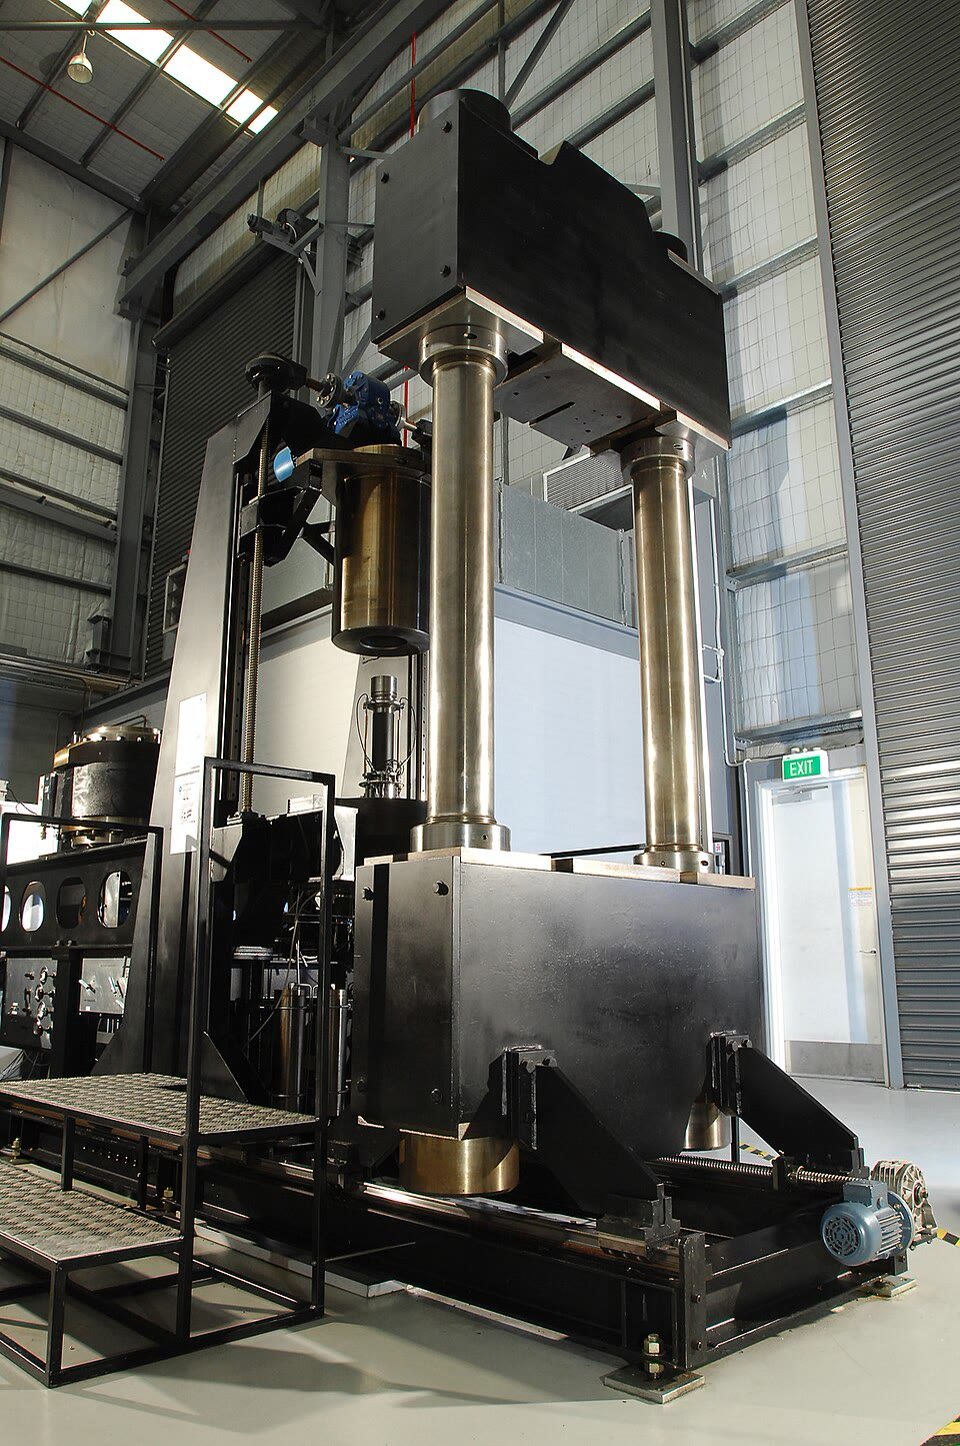
\includegraphics[width=\linewidth]{images/book3/b1-triaxial-cell.jpg}

{\scriptsize خلية ثلاثية المحاور عالية الضغط لقياس متانة الصخر
(Darryl Peroni, CSIRO, CC BY 3.0).}
% ledger: commons:csiro-triaxial
\end{minipage}
\end{inthelab}

\section{قوّة الغلاف الصخري}\label{sec:b1:stress-strain-rheology:envelope}

على كل عمق يمكن أن ينهار \omterm{def:b1:layered-earth:lithosphere}{الغلاف الصخري} بطريقتين: بالانزلاق على الصدوع، بمقاومة تتزايد مع الضغط الفعّال، أو بالزحف، بمقاومة تنخفض كلما اشتدّت الحرارة. وهو يتشوّه بالطريقة التي تحتاج إلى الإجهاد الأصغر.

\begin{definition}[غلاف المتانة، والانتقال الهشّ--اللدن، والطبقة المولّدة للزلازل]\label{def:b1:stress-strain-rheology:strength-envelope}
\emph{غلاف المتانة}\index{غلاف المتانة} \omterm{def:b1:layered-earth:lithosphere}{للغلاف الصخري} هو المنحنى، بدلالة العمق، لأكبر إجهاد تفاضلي يتحمّله عند معدّل انفعال معيّن: على كل عمق، الأصغر من المتانة الاحتكاكية ومتانة الزحف. و\emph{الانتقال الهشّ--اللدن}\index{الانتقال الهشّ--اللدن} هو العمق الذي تتساوى عنده الاثنتان: فوقه يتشوّه الصخر بالصدوع، وتحته بالزحف. و\emph{الطبقة المولّدة للزلازل}\index{الطبقة المولّدة للزلازل} هي نطاق الأعماق التي تبدأ فيها أغلب الزلازل.
\end{definition}

\begin{proposition}[المتانة الاحتكاكية بدلالة العمق]\label{prop:b1:stress-strain-rheology:brittle-gradient}
في طبقة كثافتها $\rho$ مع ضغط مسام هيدروستاتيكي، وإجهاد رئيسي واحد شاقولي، وصدوع من كل اتجاه ودون تماسك، يبدأ الانزلاق باحتكاك $\mu$ عند \omterm{def:b1:stress-strain-rheology:principal}{الإجهاد التفاضلي}
\begin{align*}
  \sigma_1 - \sigma_3 &= \frac{2\mu}{\sqrt{1+\mu^2} + \mu}\,\rho g z(1-\lambda)
  && \text{إذا كان $\sigma_v = \sigma_1$}, \\
  \sigma_1 - \sigma_3 &= \frac{2\mu}{\sqrt{1+\mu^2} - \mu}\,\rho g z(1-\lambda)
  && \text{إذا كان $\sigma_v = \sigma_3$},
\end{align*}
مع $\lambda = \rho_w/\rho$: الحالة الأولى تعطي الصدوع العادية، والثانية الصدوع الدفعية.
\end{proposition}

\begin{proof}
\omterm{def:b1:stress-strain-rheology:lithostatic}{الإجهاد الفعّال} الشاقولي هو $S = \rho g z - \rho_w g z = \rho g z(1-\lambda)$.
مع $C = 0$ و$k = \sqrt{1+\mu^2}$، تقول \cref{thm:b1:stress-strain-rheology:failure-angle} إن الصدع ينزلق حين $r = \mu c'/k$، حيث $r$ نصف القطر و$c'$ المركز لدائرة موهر الفعّالة. فإذا كان $\sigma_v = \sigma_1$، فإن $\sigma_1' = S$ و$c' = S - r$، أي $rk = \mu S - \mu r$ و$r = \mu S/(k+\mu)$. وإذا كان $\sigma_v = \sigma_3$، فإن $c' = S + r$ و$r = \mu S/(k-\mu)$. \omterm{def:b1:stress-strain-rheology:principal}{والإجهاد التفاضلي} هو $2r$.
\end{proof}

مع $\mu = 0.85$ و$\rho = \qty{2700}{kg.m^{-3}}$ يزداد $S$ بمقدار \qty{16.7}{MPa} لكل كيلومتر، ويزداد الاحتكاك بمقدار \qty{13.1}{MPa} لكل كيلومتر تحت الشدّ، و\qty{61.3}{MPa} لكل كيلومتر تحت الضغط، أي نحو خمسة أضعاف: \omterm{def:b1:layered-earth:layers}{فالقشرة} أسهل بكثير أن تُسحب من أن تُدفع معًا. وفوق إجهاد عمودي فعّال مقداره \qty{200}{MPa} يحلّ الفرع العلوي من \omterm{prop:b1:stress-strain-rheology:byerlee}{قانون بايرلي}، فينخفض الميل، تحت الضغط، إلى نحو \qty{35}{MPa} لكل كيلومتر.
% computed in figdata/bachelor-1/strength_envelope.py (tested); ledger: byerlee:1975

\begin{omfigure}
\begin{tikzpicture}
\pgfplotsset{envaxis/.style={omrecord, omdepth, scale only axis, width=5.6cm, height=7.2cm,
  xmin=-1000, xmax=2500, ymin=0, ymax=80, xtick={-1000,0,1000,2000},
  ytick={0,10,...,80}, unbounded coords=jump,
  xlabel={الإجهاد التفاضلي $\sigma_1-\sigma_3$ (\unit{MPa})},
  tick label style={font=\scriptsize}, label style={font=\small},
  scaled x ticks=false, xticklabel style={/pgf/number format/.cd, 1000 sep={\,}}}}
% computed in figdata/bachelor-1/strength_envelope.py; ledger: byerlee:1975, lopez:flow-laws, codata:R, prem:moho-average
\begin{axis}[envaxis, name=cont, ylabel={العمق (\unit{km})}, title={\small (أ) قارة, \qty{55}{mW.m^{-2}}}]
\addplot[fill=omLithGranite!45, draw=none] table[x=x, y=depth] {figdata/out/bachelor-1-strength_envelope-continental-outline.dat};
\addplot[omThm, line width=0.5pt, restrict x to domain=-1:2450] table[x=thrust, y=depth] {figdata/out/bachelor-1-strength_envelope-continental.dat};
\addplot[omThm, line width=0.5pt, restrict x to domain=-2450:1] table[x expr=-\thisrow{normal}, y=depth] {figdata/out/bachelor-1-strength_envelope-continental.dat};
\addplot[omDef, line width=0.5pt, restrict x to domain=-1:2450] table[x=ductile, y=depth] {figdata/out/bachelor-1-strength_envelope-continental.dat};
\addplot[omDef, line width=0.5pt, restrict x to domain=-2450:1] table[x expr=-\thisrow{ductile}, y=depth] {figdata/out/bachelor-1-strength_envelope-continental.dat};
\addplot[black, line width=1.0pt] table[x=x, y=depth] {figdata/out/bachelor-1-strength_envelope-continental-outline.dat};
\draw[black!60, dashed] (axis cs:-1000,35) -- (axis cs:2500,35);
\node[font=\scriptsize, anchor=south east] at (axis cs:2480,35) {موهو};
\draw[black, densely dotted] (axis cs:0,0) -- (axis cs:0,80);
\draw[black!70] (axis cs:660,13.7) -- (axis cs:1700,18) node[anchor=north, font=\scriptsize, align=center, text=black] {الانتقال\\ \qty{14}{km}};
\draw[black!70] (axis cs:1870,44.6) -- (axis cs:1950,53) node[anchor=north, font=\scriptsize, align=center, text=black] {انتقال\\ الوشاح};
\node[font=\scriptsize, anchor=north, omThm] at (axis cs:1500,3) {ضغط};
\node[font=\scriptsize, anchor=north, omThm] at (axis cs:-560,3) {شدّ};
\node[font=\scriptsize, anchor=west, omDef] at (axis cs:40,31) {كوارتز رطب};
\node[font=\scriptsize, anchor=west, omDef] at (axis cs:300,66) {أوليفين جاف};
\end{axis}
\begin{axis}[envaxis, at={(cont.east)}, anchor=west, xshift=0.6cm, yticklabels={}, title={\small (ب) قاع محيطي عمره \qty{60}{Myr}}]
\addplot[fill=omLithBasalt!45, draw=none] table[x=x, y=depth] {figdata/out/bachelor-1-strength_envelope-oceanic-outline.dat};
\addplot[omThm, line width=0.5pt, restrict x to domain=-1:2450] table[x=thrust, y=depth] {figdata/out/bachelor-1-strength_envelope-oceanic.dat};
\addplot[omThm, line width=0.5pt, restrict x to domain=-2450:1] table[x expr=-\thisrow{normal}, y=depth] {figdata/out/bachelor-1-strength_envelope-oceanic.dat};
\addplot[omDef, line width=0.5pt, restrict x to domain=-1:2450] table[x=ductile, y=depth] {figdata/out/bachelor-1-strength_envelope-oceanic.dat};
\addplot[omDef, line width=0.5pt, restrict x to domain=-2450:1] table[x expr=-\thisrow{ductile}, y=depth] {figdata/out/bachelor-1-strength_envelope-oceanic.dat};
\addplot[black, line width=1.0pt] table[x=x, y=depth] {figdata/out/bachelor-1-strength_envelope-oceanic-outline.dat};
\draw[black, densely dotted] (axis cs:0,0) -- (axis cs:0,80);
\draw[black!70] (axis cs:2003,38.2) -- (axis cs:1900,50) node[anchor=north, font=\scriptsize, align=center, text=black] {الانتقال\\ \qty{38}{km}};
\node[font=\scriptsize, anchor=west, omDef] at (axis cs:300,66) {أوليفين جاف};
\end{axis}
\end{tikzpicture}
\par\smallskip{\small أغلفة المتانة عند معدّل الانفعال \qty{e-15}{s^{-1}}. الأحمر: المتانة الاحتكاكية وفق \omterm{prop:b1:stress-strain-rheology:byerlee}{قانون بايرلي} مع ضغط مسام هيدروستاتيكي، للضغط (الصدع الدفعي، يمينًا) وللشدّ (الصدع العادي، يسارًا، ويُرسم سالبًا)؛ والأزرق: متانة الزحف للكوارتزيت الرطب في \omterm{def:b1:layered-earth:layers}{القشرة} القارية، وللأوليفين الجاف في \omterm{def:b1:layered-earth:layers}{الوشاح}؛ والخطّ الأسود والتظليل: المتانة، أي الأصغر من الاثنتين عند كل عمق. (أ) قارة يبلغ فيها التدفّق الحراري السطحي \qty{55}{mW.m^{-2}}، \omterm{def:b1:layered-earth:layers}{وقشرة} سمكها \qty{35}{km}: \omterm{def:b1:layered-earth:layers}{قشرة} علوية قوية، \omterm{def:b1:layered-earth:layers}{وقشرة} سفلى ضعيفة، \omterm{def:b1:layered-earth:layers}{ووشاح} علوي قوي. (ب) قاع محيطي عمره \qty{60}{Myr}: طبقة واحدة قوية، سمكها \qty{38}{km} تحت الضغط.}
\label{fig:b1:stress-strain-rheology:envelope}
\end{omfigure}

يجمع الشكل أعلاه المقاومتين لغلافين صخريين. فالقارة لها \omterm{def:b1:heat-budget:geotherm}{المنحنى الحراري} الوارد في \cref{ch:b1:heat-budget} مع تدفّق حراري سطحي \qty{55}{mW.m^{-2}}، \omterm{def:b1:layered-earth:layers}{وقشرة} من كوارتزيت رطب سمكها \qty{35}{km}، \omterm{def:b1:rock-forming-minerals:groups}{وأوليفين} جاف تحتها؛ وقاع المحيط عمره \qty{60}{Myr}، مع \omterm{def:b1:heat-budget:geotherm}{المنحنى الحراري} لنصف الفضاء في الفصل نفسه، \omterm{def:b1:rock-forming-minerals:groups}{والأوليفين} من قاع البحر إلى الأسفل. ومعدّل الانفعال هو \qty{e-15}{s^{-1}}. و\qty{35}{km} هو متوسط عمق \omterm{def:b1:layered-earth:discontinuity}{موهو} تحت القارات في \omterm{def:b1:layered-earth:reference-model}{نموذج الأرض المرجعي} الوارد في \cref{ch:b1:layered-earth}.
% ledger: prem:moho-average

تحت القارة ينخفض \omterm{def:b1:stress-strain-rheology:strength-envelope}{الانتقال الهشّ--اللدن} إلى \qty{13.7}{km} تحت الضغط، عند \qty{249}{\degreeCelsius}، وإلى \qty{17.1}{km} تحت الشدّ. \omterm{def:b1:layered-earth:layers}{وقشرة} أدفأ كانت سترفعه، \omterm{def:b1:layered-earth:layers}{وقشرة} أبرد تخفضه، لأن قانون الزحف يتعلّق بالحرارة وحدها عند إجهاد معيّن. والانتقال هو أقوى مستوى في \omterm{def:b1:layered-earth:layers}{القشرة}.
وتحته تنهار المتانة: عند \omterm{def:b1:layered-earth:discontinuity}{موهو}، عند \qty{527}{\degreeCelsius}، ينساب الكوارتزيت تحت \qty{7.6}{MPa}، بينما يحتاج \omterm{def:b1:rock-forming-minerals:groups}{الأوليفين} عند الحرارة نفسها إلى نحو \qty{30000}{MPa}، أي أبعد بكثير من المتانة الاحتكاكية، فيصير أعلى \omterm{def:b1:layered-earth:layers}{الوشاح} هشًّا من جديد. ويليه انتقال ثانٍ عند \qty{44.6}{km} تحت الضغط. \omterm{def:b1:layered-earth:layers}{والقشرة} السفلى في هذا النموذج طبقة ليّنة بين طبقتين قويتين: «ساندويتش الهلام». أما تحت المحيط \omterm{def:b1:layered-earth:lithosphere}{فالغلاف الصخري} كله \omterm{def:b1:rock-forming-minerals:groups}{أوليفين}، وتزداد المتانة نزولًا حتى انتقال واحد عند \qty{38.2}{km}، عند \qty{641}{\degreeCelsius}.
% computed in figdata/bachelor-1/strength_envelope.py (tested)

تتّفق الزلازل مع المغلّف المحيطي: داخل الصفائح المحيطية تبلغ الأعماق التي تكون فيها الحرارة \qtyrange{600}{800}{\degreeCelsius}، قريبًا من \qty{641}{\degreeCelsius} وهي حرارة الانتقال الوحيد في النموذج. والزلازل الأعمق لا تقع إلا حيث تغوص صفيحة تحت أخرى، حتى عمق يزيد على \qty{700}{km} (\cref{ch:b1:active-margins}).
% ledger: jackson:jelly, usgs:deepest

وفي \omterm{def:b1:layered-earth:layers}{الوشاح} القاري تبقى الصورة موضع نزاع. فلنحو عشرين سنة كان «ساندويتش الهلام» هو الرأي السائد، استنادًا إلى قياسات مخبرية على \omterm{def:b1:rock-forming-minerals:groups}{الأوليفين} الجاف وإلى زلازل قليلة يُظنّ أنها تقع تحت \omterm{def:b1:layered-earth:discontinuity}{موهو}. وفي 2002 رأى جيمس جاكسون أنه يجب التخلّي عنه: فقد أظهرت تحديدات أفضل للأعماق أن الزلازل في القارات محصورة في طبقة واحدة، عادةً \omterm{def:b1:layered-earth:layers}{القشرة} العليا، وأحيانًا \omterm{def:b1:layered-earth:layers}{القشرة} كلها، دون زلازل مقنعة في \omterm{def:b1:layered-earth:layers}{الوشاح} تحتها، حتى حيث يكون \omterm{def:b1:layered-earth:discontinuity}{موهو} عند \qtyrange{300}{500}{\degreeCelsius} فقط. وكميات صغيرة من الماء، بضعة أجزاء في المليون في \omterm{def:b1:rock-forming-minerals:groups}{الأوليفين}، تكفي لإضعافه إضعافًا شديدًا، وقد يحمل \omterm{def:b1:layered-earth:layers}{الوشاح} القاري قدرًا كهذا؛ فتكون متانة القارات عندئذ كامنة في قشرتها أساسًا. والرأيان يرسمان مغلّفين مختلفين من القوانين نفسها، مع \omterm{def:b1:rock-forming-minerals:groups}{أوليفين} جاف أو رطب تحت \omterm{def:b1:layered-earth:discontinuity}{موهو}.
% ledger: jackson:jelly
وأيًّا كان الصحيح، فالمغلّف حدّ وليس قياسًا: فقوانين المختبر تُستقرأ عبر عدّة مراتب من الكبر في معدّل الانفعال، والإجهادات القصوى التي يُظهرها، أكثر من غيغاباسكال، أعلى بكثير من \qtyrange{1}{10}{MPa} التي تُلاحظ الزلازل أنها تطلقها.
% ledger: jackson:jelly

\section{التمارين}

\begin{exercise}[$\star$]\label{exo:b1:stress-strain-rheology:1}
خذ \omterm{def:b1:layered-earth:layers}{قشرة} كثافتها \qty{2700}{kg.m^{-3}} و$g = \qty{9.81}{m.s^{-2}}$. على عمق \qty{10}{km} احسب (أ) الإجهاد الشاقولي، (ب) ضغط المسام الهيدروستاتيكي، (ج) \omterm{def:b1:stress-strain-rheology:lithostatic}{الإجهاد الفعّال} الشاقولي ونسبة ضغط المسام $\lambda$.
\end{exercise}

\begin{exercise}[$\star$]\label{exo:b1:stress-strain-rheology:2}
(أ) تُمدّ طبقة طولها \qty{10}{km} حتى \qty{13}{km}: أعطِ استطالتها ومطّها. (ب) طبقة أخرى طولها \qty{10}{km} تُقصَّر إلى \qty{7}{km}. (ج) خطّان من صخر كانا متعامدين صارا يصنعان الآن زاوية \ang{60}: ما القصّ الزاوي \omterm{def:b1:stress-strain-rheology:strain}{وانفعال القصّ}؟
\end{exercise}

\begin{exercise}[$\star$]\label{exo:b1:stress-strain-rheology:3}
عند نقطة، $\sigma_1 = \qty{100}{MPa}$ و$\sigma_3 = \qty{40}{MPa}$. (أ) ارسم دائرة موهر. (ب) ما أكبر إجهاد قصّ، وعلى أيّ مستويات يؤثّر، وأيّ إجهاد عمودي يؤثّر عليها؟ (ج) احسب $\sigma_n$ و$\tau$ على المستوى الذي يصنع عموده الزاوية \ang{30} مع $\sigma_1$.
\end{exercise}

\begin{exercise}[$\star$]\label{exo:b1:stress-strain-rheology:4}
تملك الصخرة تماسكًا قدره \qty{10}{MPa}، وزاوية احتكاك داخلي قدرها \ang{30}. (أ) عند أي زاوية مع $\sigma_1$ تنكسر، وما الزاوية التي تصنعها المستويان الممكنان للكسر مع بعضهما؟ (ب) مع $\sigma_3' = \qty{20}{MPa}$، ما \omterm{def:b1:stress-strain-rheology:lithostatic}{الإجهاد الفعّال} $\sigma_1'$ الذي يكسرها؟
\end{exercise}

\begin{exercise}[$\star\star$]\label{exo:b1:stress-strain-rheology:5}
في المحورين $x$ (الأفقي) و$y$ (الشاقولي)، $\sigma_{xx} = \qty{60}{MPa}$، و$\sigma_{yy} = \qty{20}{MPa}$، و$\sigma_{xy} = \qty{15}{MPa}$. (أ) احسب \omterm{def:b1:stress-strain-rheology:principal}{الإجهادات الرئيسية} والزاوية $\theta_p$. (ب) تحقّق ب\cref{prop:b1:stress-strain-rheology:transformation} أن المستوى الذي عموده $\theta_p$ لا يحمل إجهاد قصّ، وأن إجهاده العمودي هو $\sigma_1$. (ج) ما أكبر إجهاد قصّ عند هذه النقطة؟
\end{exercise}

\begin{exercise}[$\star\star$]\label{exo:b1:stress-strain-rheology:6}
عملت منطقة قصّ على تشويه صخرها بقصّ بسيط $\gamma = 2$. (أ) احسب المطّين الرئيسيين، وزاوية المحور الطويل للقطع الناقص للانفعال مع اتجاه القصّ. (ب) تحقّق أن المساحة لم تتغيّر. (ج) خطّ مادي كان يصنع \ang{45} مع اتجاه القصّ، ويصعد في اتجاهه: أين يقع الآن، وما مطّه؟ قارن ذلك ب(أ).
\end{exercise}

\begin{exercise}[$\star\star$]\label{exo:b1:stress-strain-rheology:7}
في منطقة قصّ سمكها \qty{200}{m}، أصبحت بقع دائرية صغيرة في الأردواز قطوعًا ناقصة نسبة محاورها 4 إلى 1. افترض قصًّا بسيطًا دون تغيّر في المساحة. (أ) أوجد $S_1$ و$S_2$ و$\gamma$. (ب) عند أي زاوية مع جدران المنطقة ينبغي أن تقع المحاور الطويلة؟ (ج) إلى أي مدى تحرّك أحد الجدران متجاوزًا الآخر؟
\end{exercise}

\begin{exercise}[$\star\star$]\label{exo:b1:stress-strain-rheology:8}
صدع على عمق \qty{3}{km}، في \omterm{def:b1:layered-earth:layers}{قشرة} كثافتها \qty{2700}{kg.m^{-3}}، يحمل إجهادًا عموديًّا قدره \qty{70}{MPa} وإجهاد قصّ قدره \qty{30}{MPa}. (أ) مع ضغط مسام هيدروستاتيكي، هل ينزلق وفق \omterm{prop:b1:stress-strain-rheology:byerlee}{قانون بايرلي}؟ (ب) وإذا كانت المسامّ مغلقة و$\lambda = 0.6$؟ (ج) أوجد قيمة $\lambda$ التي يبدأ عندها الانزلاق.
\end{exercise}

\begin{exercise}[$\star\star$]\label{exo:b1:stress-strain-rheology:9}
استعمل قانون الزحف للكوارتزيت الرطب (\cref{prop:b1:stress-strain-rheology:creep}). (أ) بأي عامل يجب أن يرتفع الإجهاد ليجري أسرع عشر مرات؟ (ب) بأي عامل تنخفض متانته بين \qty{400}{\degreeCelsius} و\qty{500}{\degreeCelsius}، عند المعدّل نفسه ومع $V = 0$؟ (ج) فسّر بهاتين النتيجتين لماذا يتعلّق عمق \omterm{def:b1:stress-strain-rheology:strength-envelope}{الانتقال الهشّ--اللدن} \omterm{def:b1:heat-budget:geotherm}{بالمنحنى الحراري} أكثر بكثير من تعلّقه بمعدّل الانفعال.
\end{exercise}

\begin{exercise}[$\star\star\star$]\label{exo:b1:stress-strain-rheology:10}
حيث يكون الإجهاد الشاقولي هو $\sigma_2$، تكون الصدوع انزياحية أفقية. افترض أن \omterm{def:b1:stress-strain-rheology:lithostatic}{الإجهاد الفعّال} الشاقولي عندئذٍ هو المتوسط $(\sigma_1' + \sigma_3')/2$. (أ) بيّن أن الانزلاق باحتكاك $\mu$ دون تماسك يبدأ عند
$\sigma_1 - \sigma_3 = 2\mu\,\rho g z(1-\lambda)/\sqrt{1+\mu^2}$. (ب) احسب الميل بالميغاباسكال لكل كيلومتر من أجل $\mu = 0.85$ و
$\rho = \qty{2700}{kg.m^{-3}}$، وضعه بين ميلي الصدع العادي والصدع الدفعي. (ج) عبّر عن كل من الأميال الثلاثة كمضاعف للإجهاد الفعّال الشاقولي.
\end{exercise}

\begin{exercise}[$\star\star\star$]\label{exo:b1:stress-strain-rheology:11}
انمذج \omterm{def:b1:layered-earth:lithosphere}{الغلاف الصخري} المحيطي عمره \qty{60}{Myr} كنصف فضاء بُرِّد من \qty{1350}{\degreeCelsius}، مع سطح عند \qty{0}{\degreeCelsius} و$\kappa = \qty{e-6}{m^2.s^{-1}}$: $T = \num{1350}\operatorname{erf}\bigl(z/(2\sqrt{\kappa t})\bigr)$. (أ) احسب $2\sqrt{\kappa t}$. (ب) أوجد أعماق متساوي الحرارة \qty{600}{\degreeCelsius} و\qty{800}{\degreeCelsius}. (ج) تبلغ الزلازل داخل الصفائح المحيطية الأعماق التي تكون فيها الحرارة \qtyrange{600}{800}{\degreeCelsius}. قارن ذلك \omterm{def:b1:stress-strain-rheology:strength-envelope}{بالانتقال الهشّ--اللدن} في \omterm{def:b1:stress-strain-rheology:strength-envelope}{غلاف المتانة} المحيطي في هذا الفصل، عند \qty{38.2}{km} و\qty{641}{\degreeCelsius}.
% ledger: jackson:jelly
\end{exercise}

\begin{exercise}[$\star\star\star$]\label{exo:b1:stress-strain-rheology:12}
يقطع صخرًا كسور من كل اتجاه، تحتوي كلها اتجاه $\sigma_2$، دون تماسك واحتكاك 0.85. \omterm{def:b1:stress-strain-rheology:principal}{والإجهادات الرئيسية} الفعّالة هي $\sigma_1' = \qty{110}{MPa}$ و$\sigma_3' = \qty{20}{MPa}$. (أ) بيّن أن بعض الكسور ينزلق. (ب) أوجد مدى الزاوية بين الكسور المنزلقة و$\sigma_1$. أيّها يقع في وسط المدى؟ (ج) حتى أي قيمة ل$\sigma_1'$، مع تثبيت $\sigma_3'$، يبقى كسر واحد على الأقل ينزلق؟
\end{exercise}

\section{مسألة: هل سينزلق الصدع؟}

\begin{problem}[{مسألة نهاية الأسبوع: الإجهاد على صدع عادي عند عمق خمسة كيلومترات، وهامش أمانه، وارتفاع ضغط المسام الذي يجعله ينزلق}]
\label{pb:b1:stress-strain-rheology:1}
% values: calc/ch16.py; ledger: byerlee:1975, hb81:denver
يمتدّ الصدع شمال--جنوب وينحدر بزاوية \ang{60} نحو الشرق. تبلغه بئر تصريف على عمق \qty{5.00}{km}، في \omterm{def:b1:layered-earth:layers}{قشرة} كثافتها \qty{2700}{kg.m^{-3}} تتّصل مسامّها بالسطح. ويعطي قياس في البئر الإجهاد الأفقي العمودي على الصدع، \qty{75.0}{MPa}؛ والإجهاد الأفقي على طول \omterm{def:b1:geological-maps:attitude}{الامتداد} يقع بينه وبين الإجهاد الشاقولي، فالمسألة ثنائية البعد في المستوى الشاقولي شرق--غرب. خذ $g = \qty{9.81}{m.s^{-2}}$، وماءً كثافته \qty{1000}{kg.m^{-3}}، \omterm{prop:b1:stress-strain-rheology:byerlee}{وقانون بايرلي}. أعطِ الإجهادات حتى \qty{0.01}{MPa}.

\medskip
\noindent\textbf{الجزء الأول --- حالة الإجهاد.}
\begin{enumerate}
  \item احسب الإجهاد الشاقولي عند عمق الصدع.
  \item احسب ضغط المسام الهيدروستاتيكي هناك، ونسبة $\lambda$.
  \item أيّ الإجهادين هو $\sigma_1$ وأيّهما $\sigma_3$؟ وأيّ نوع من الصدوع تقود إليه حالة الإجهاد هذه؟
  \item احسب \omterm{def:b1:stress-strain-rheology:principal}{الإجهاد التفاضلي}، ومركز دائرة موهر ونصف قطرها.
  \item احسب \omterm{def:b1:stress-strain-rheology:principal}{الإجهادات الرئيسية} الفعّالة، ومركز الدائرة الفعّالة.
  \item مع كون $x$ أفقيًّا نحو الشرق و$y$ شاقوليًّا، اكتب المركّبات الثلاث $\sigma_{xx}$ و$\sigma_{yy}$ و$\sigma_{xy}$. لماذا يكون $\sigma_{xy}$ معدومًا؟
\end{enumerate}

\medskip
\noindent\textbf{الجزء الثاني --- الإجهادات على الصدع.}
\begin{enumerate}[resume]
  \item أعطِ المتجهة الوحدة العمودية على الصدع في محاور السؤال 6، والزاوية $\theta$ بينها وبين $\sigma_1$.
  \item احسب $\sigma_n$ و$\tau$ على الصدع ب\cref{prop:b1:stress-strain-rheology:transformation}.
  \item تحقّق من القيمتين بدائرة موهر: عند أي زاوية من طرف $\sigma_1$ يقع الصدع؟
  \item احسب \omterm{def:b1:stress-strain-rheology:stress}{الإجهاد العمودي} الفعّال على الصدع.
  \item احسب النسبة $\tau/\sigma_n'$ وقارنها بالقيمة 0.85.
  \item ما إجهاد القصّ الذي يجعل الصدع ينزلق تحت \omterm{def:b1:stress-strain-rheology:stress}{الإجهاد العمودي} الفعّال الحالي؟ بكم ميغاباسكال يقصر عنه؟
\end{enumerate}

\medskip
\noindent\textbf{الجزء الثالث --- دائرة موهر \omterm{prop:b1:stress-strain-rheology:byerlee}{وقانون بايرلي}.}
\begin{enumerate}[resume]
  \item ارسم دائرة موهر الفعّالة وخطّ بايرلي بالمقياس.
  \item احسب المسافة من مركز الدائرة إلى الخطّ وقارنها بنصف القطر. هل يستطيع أي مستوٍ يمرّ بالصخر أن ينزلق؟
  \item أيّ مستوٍ سينزلق أولًا؟ أعطِ زاويته مع $\sigma_1$ وانحداره.
  \item باستعمال \cref{prop:b1:stress-strain-rheology:brittle-gradient}، احسب \omterm{def:b1:stress-strain-rheology:principal}{الإجهاد التفاضلي} الذي تنزلق عنده الصدوع العادية على هذا العمق، وقارنه بميل \qty{13.1}{MPa} لكل كيلومتر.
  \item كم يجب أن ينخفض الإجهاد الأفقي حتى ينزلق المستوي الأفضل توجّهًا؟
  \item كم يجب أن ينخفض حتى ينزلق صدع المسألة؟ اشرح لماذا يكون أدنى.
\end{enumerate}

\medskip
\noindent\textbf{الجزء الرابع --- الحقن.}
\begin{enumerate}[resume]
  \item اشرح لماذا يحرّك ارتفاعُ ضغط المسام $\Delta P$ الدائرةَ الفعّالة بمقدار $\Delta P$ نحو اليسار دون أن يغيّر نصف قطرها.
  \item احسب ارتفاع ضغط المسام الذي يجعل المستوي الأفضل توجّهًا ينزلق.
  \item البئر مملوءة بالماء. ما الضغط الإضافي الذي يجب أن تطبّقه المضخة عند رأس البئر لرفع ضغط المسام عند الصدع بذلك المقدار؟ وكم يعادل من عمود ماء؟
  \item لو كان احتكاك الصدع 0.6 بدلًا من 0.85، هل كان سينزلق من قبل؟ ماذا يقول سكون الصدع عن احتكاكه؟
  \item عند أي نسبة $\lambda$ ينزلق المستوي الأفضل توجّهًا؟
  \item إلى رقم عشري واحد، وبالميغاباسكال، أي ارتفاع في ضغط المسام يجعل هذا الصدع ينزلق؟
\end{enumerate}
\end{problem}
